\pstart\noindent\hangindent=10mm\hspace{10mm}Difficultas Machinae Hydrographicae\protect\index{Sachverzeichnis}{machina!hydrographica} in distantiis exhibendis ideo magna est, quia aqua non est stabilis et quieta, ita ut navis\protect\index{Sachverzeichnis}{navis} in ea feratur, ut currus in terra. Et aqua saepe persequitur navem\protect\index{Sachverzeichnis}{navis}, ut quando ab ejus currente fertur non ergo tunc aqua rotas\protect\index{Sachverzeichnis}{rota} circumagens discrimen dabit, adde quod currentes modo adversi modo secundi, modo obliqui, haec omnia turbant.\footnote{\textit{In der rechten Spalte}:\\
 \protect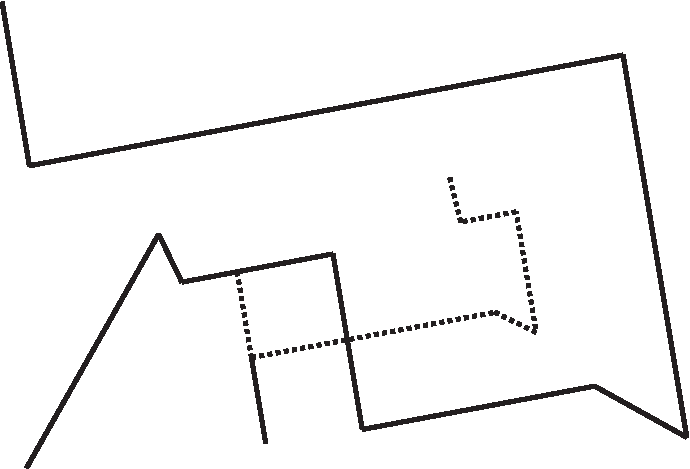
\includegraphics[width=0.2\textwidth]{images/LH38_18v_2}
 %\\\hspace{15mm} [\textit{Fig. 2}]
NB Solis flexibus cognitis, nisi detur distantia inter flexus, non linea motus, sed ejus parallela invenitur. Quae jam tam (demto declinationis\protect\index{Sachverzeichnis}{declinatio} errore) semper nota est, angulus scilicet, quem faciat navis\protect\index{Sachverzeichnis}{navis} motus ad plagas mundi. Ergo solis istis flexibus sola invenitur declinatio\protect\index{Sachverzeichnis}{declinatio}, quod non est tanti, nisi continue ipsa se machina adhibitis non flexibus tantum sed et intervallis emendet.}
Idem est in ventis, nam et venti sunt aeris currentes. Aestimari posset instrumentis certis quae sit vis venti in navem\protect\index{Sachverzeichnis}{navis}, data obliquitate, datoque velorum positu, ita aestimari posset celeritas\protect\index{Sachverzeichnis}{celeritas} cursus navis\protect\index{Sachverzeichnis}{navis} ex calculo; et fateor hanc aestimationem dignam exquiri, caeterisque addendam; sed tamen currentium \edtext{complicatio}{\lemma{currentium}\Afootnote{ \textit{ (1) }\ consideratio \textit{ (2) }\ complicatio \textit{ L}}} rem perturbat. Posset projici aliquid ante navem\protect\index{Sachverzeichnis}{navis}, in linea cursus, quod assequamur, aut relinqui quod attrahamus. Idque saepe repeti, aut saltem quamdiu ex omnibus apparet idem rerum status semel, atque inde fieri aestimatio. Sed haec omnia per incommoda, atque incerta.\newline Crediderim etiam cum \edtext{ventus impellit navem, non tamen}{\lemma{ventus}\Afootnote{ \textit{ (1) }\ non fert, ta \textit{ (2) }\ impellit navem, non tamen \textit{ L}}} portare, et ideo nave\protect\index{Sachverzeichnis}{navis} licet secundo vento provehente aeris tamen sibilum in contrarium esse posse in canali. Sed quomodo\edtext{ sibilans aer egredietur canali contra ventum: an dabimus ei exitum in navem}{\lemma{quomodo}\Afootnote{ \textit{ (1) }\ navis \textit{ (2) }\ sibilans [...] navem \textit{ L}}}. Hoc optimum. Sed videtur totus aer impelli cum nave\protect\index{Sachverzeichnis}{navis}, unde et sagitta relabens. Ergo et aqua eodem \edtext{modo, superficiaria}{\lemma{modo,}\Afootnote{ \textit{ (1) }\ ut \textit{ (2) }\ superficiaria \textit{ L}}} inprimis nonnihil sequitur navem\protect\index{Sachverzeichnis}{navis}. Et omnino si navis\protect\index{Sachverzeichnis}{navis} quodammodo currente feratur, illud \hspace{1mm}tamen observandum: \hspace{1mm}quando \hspace{1mm}currens \hspace{1mm}fert \hspace{1mm}navem, ex aere,\pend\pstart\noindent\hangindent=10mm\hspace{10mm}quando ventus ex aqua nonnihil sciri posse celeritatem\protect\index{Sachverzeichnis}{celeritas}, praesertim si utrobique machina talis sit ut non nisi motu conspirante feratur. Quod fiet si sit machina, in qua omnis actio in contrarium seu reactio rotarum\protect\index{Sachverzeichnis}{rota} impediatur etiam aperta communicatione, ut \protect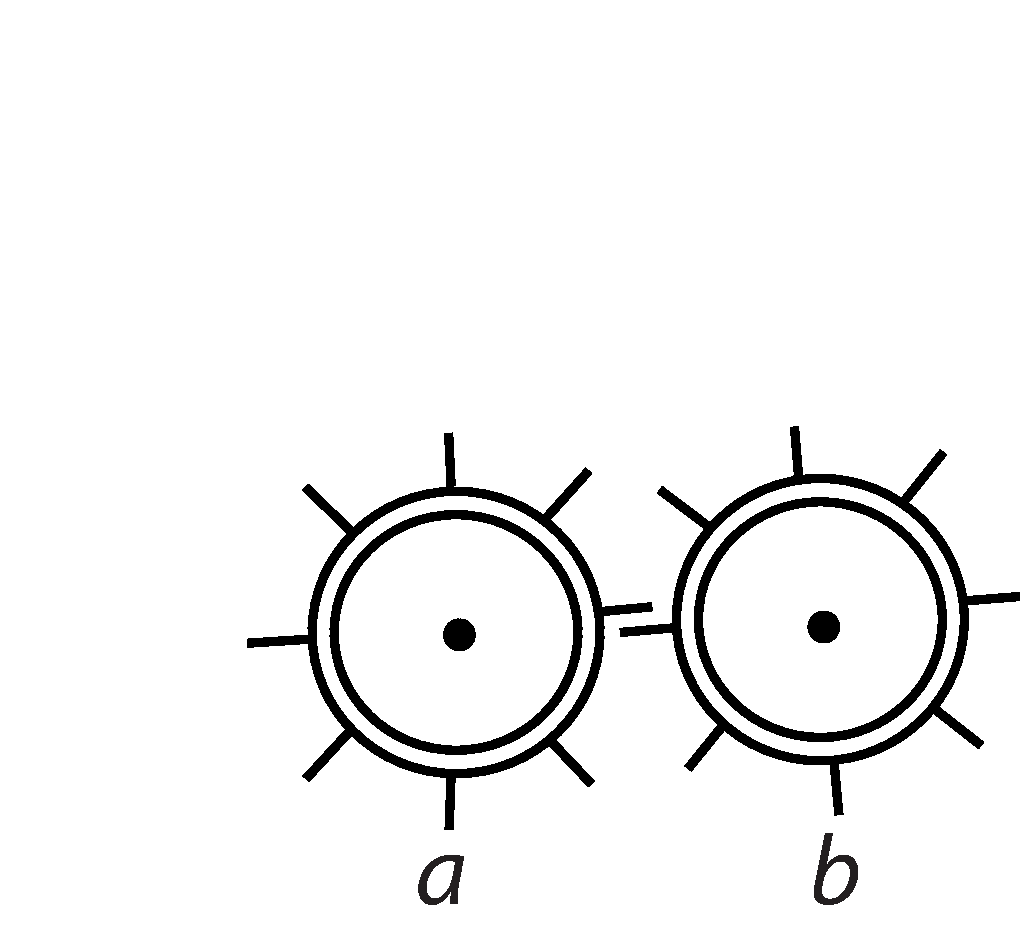
\includegraphics[width=0.1\textwidth]{images/38_18v2} ex. g. rota\protect\index{Sachverzeichnis}{rota} \textit{a} accipiat actionem a \textit{b} et tamen si quis impetus agere velit in \textit{a} momento etiam motus vel porro vel retro agendo nonnihil non possit etsi fortissimus.\footnote{\textit{In der rechten Spalte}: Quod ita tento: Ante omnia facile fiet, ut rota \textit{b} possit quidem progredi sed non regredi. Et per consequens etiam rota \protect\index{Sachverzeichnis}{rota}\textit{a}. Sed ut rota \protect\index{Sachverzeichnis}{rota}\textit{a} ne ire quidem celerius possit, quam impetus impellit a rota \protect\index{Sachverzeichnis}{rota}\textit{b} quod efficiemus. Ecce modum qui mihi in mentem venit.
% \protect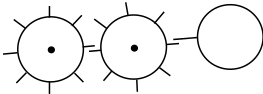
\includegraphics[width=0.3\textwidth]{images/38_18v3} 
 %\\\hspace{15mm}[\textit{Fig. 3}]
} \pend